\documentclass[11pt,a4paper]{article}

\usepackage[T1]{fontenc}
\usepackage{lmodern}
\usepackage{microtype}
\usepackage[margin=2.5cm]{geometry}
\usepackage{amsmath,amssymb}
\usepackage{booktabs}
\usepackage{graphicx}
\usepackage{caption}
\usepackage{siunitx}
\usepackage[authoryear,round]{natbib}
\usepackage{xurl}
\usepackage[hidelinks]{hyperref}
\usepackage{setspace}
\setstretch{1.12}
\captionsetup{font=small,labelfont=bf}
\sisetup{detect-all}

\title{Does Calibration Pay? Calibration-Optimised and Accuracy-Optimised Classifiers in a Monthly Equity Outperformance Strategy}
\author{Pablo Williams\thanks{Independent researcher, London, United Kingdom. Email: \texttt{pablowilliams119@gmail.com}. An earlier version of this work was prepared during the author's MSc studies. The analysis, code and conclusions are the author's own, as are any errors. Code and outputs: \url{https://github.com/pablowilliams/calibration-portfolio}.}}
\date{November 2026\\[0.3em]\small Working paper. Comments welcome.}

\begin{document}
\maketitle

\begin{abstract}
\noindent
When a classifier's predicted probabilities are used to size positions, the quality of those probabilities matters as much as the ranking they imply. This paper asks whether selecting a model for calibration rather than for accuracy produces a better portfolio. Using 82{,}260 stock-months for 457 S\&P~500 constituents from 2010 to 2024, I predict whether each stock will outperform the SPY index fund in the following month from 20 lagged features: technical indicators, Elo-style relative-strength ratings, Bayesian shrinkage estimates of expected return, and macroeconomic variables. Six classifiers are tuned with an expected calibration error (ECE) objective under temporal cross-validation. The best-calibrated model (a random forest, validation ECE 0.026) and the most accurate model (XGBoost, validation accuracy 50.4\%) each drive a half-Kelly portfolio, rebalanced monthly with transaction costs, over an untouched 2021 to 2024 test period. The calibration-selected portfolio returned 68.1\% against 63.4\%, with a Sharpe ratio of 0.77 against 0.71. The difference is not statistically significant (paired $t(47)=0.545$, one-sided $p=0.294$; bootstrap 95\% interval for the Sharpe difference $[-0.080, 0.204]$), and neither portfolio beat an equal-weighted portfolio of the same stocks (Sharpe 0.82) or the SPY exchange-traded fund (0.83). Discrimination was close to chance throughout (test AUC 0.48 to 0.50). The main finding is therefore negative but informative: with a signal this weak, calibration error mostly measures how closely predictions hug the base rate, and selecting on it does not produce a reliable economic gain.
\end{abstract}

\noindent\textbf{Keywords:} probability calibration; expected calibration error; Kelly criterion; cross-sectional return prediction; model selection; machine learning in finance\\
\textbf{JEL codes:} C45, C52, G11, G17

\section{Introduction}

Most applications of machine learning to return prediction choose models by accuracy, area under the ROC curve, or a ranking metric \citep{gu2020}. Those metrics reward a model for ordering stocks correctly. They say nothing about whether a predicted probability of 0.60 corresponds to a stock that outperforms 60\% of the time. For a portfolio that only uses ranks, this does not matter. For a portfolio that sizes positions from the probabilities themselves, as Kelly-type rules do \citep{kelly1956,thorp2006}, a miscalibrated probability translates directly into a mis-sized bet.

This gives a simple, testable claim. If position sizes depend on predicted probabilities, then a model chosen for calibration should produce better risk-adjusted returns than a model chosen for accuracy, even if the second model is slightly better at classification. The idea is well established in the forecasting literature \citep{brier1950,murphy1973} and in machine learning, where modern classifiers are known to be miscalibrated in systematic ways \citep{niculescu2005,guo2017}. It has received less direct testing in equity portfolio construction.

This paper runs that test on a deliberately transparent pipeline. It makes three contributions.
\begin{enumerate}
  \item It compares a calibration-selected and an accuracy-selected classifier under an identical position-sizing rule, so that the difference between the two portfolios isolates the effect of the selection criterion.
  \item It reports the result with formal inference and with the benchmarks that a practitioner would ask for, including equal weighting \citep{demiguel2009}, rather than against a zero return.
  \item It documents why the result is null. With discrimination close to chance, predicted probabilities collapse into a narrow band around the base rate, and the expected calibration error then rewards conservatism rather than useful information.
\end{enumerate}

The answer is that calibration did not pay in a statistically detectable way. The calibration-selected portfolio earned more than the accuracy-selected one, by 4.7 percentage points over four years, but the paired test cannot distinguish that gap from noise and both portfolios lagged simple benchmarks. I report this as the central result rather than as a failure, because a clearly documented negative result on a plausible hypothesis is useful to anyone considering the same design.

\section{Related work}

\paragraph{Calibration.} A forecaster is calibrated if, among all occasions on which it predicts probability $p$, the event occurs with frequency $p$. The Brier score \citep{brier1950} and its decomposition into reliability, resolution and uncertainty \citep{murphy1973} remain the standard tools. \citet{niculescu2005} showed that boosted trees and support vector machines push probabilities away from the extremes while bagged trees and neural networks behave differently, and \citet{guo2017} showed that deep networks tend to be overconfident. Post-hoc corrections such as Platt scaling \citep{platt1999} and isotonic regression \citep{zadrozny2002} are common. The expected calibration error, a binned summary of reliability, is widely used for model comparison \citep{naeini2015} despite known sensitivity to binning.

\paragraph{Probabilities and position sizing.} The Kelly criterion maximises long-run growth when the probability of a favourable outcome is known \citep{kelly1956}. In practice the probability is estimated, and fractional Kelly rules are used to limit the damage done by estimation error \citep{thorp2006,maclean2011}. This is the mechanism through which calibration should matter: the stake is a function of the probability, so an error in the probability becomes an error in the stake.

\paragraph{Machine learning for returns.} \citet{gu2020} find that tree ensembles and neural networks improve cross-sectional return prediction over linear models, with gains concentrated in nonlinear interactions. A large literature warns that apparent predictability often reflects data mining, look-ahead or survivorship \citep{harvey2016,bailey2014,lopezdeprado2018}. Equal weighting is a demanding benchmark for any optimised portfolio \citep{demiguel2009}.

\paragraph{Ratings and shrinkage.} Elo ratings were designed for paired comparisons in chess \citep{elo1978} and have been applied to many settings in which a running estimate of relative strength is updated from wins and losses. Shrinking noisy individual estimates toward a group mean is the classic empirical Bayes result of \citet{efron1977}. Both are used here as feature constructions rather than as models in their own right.

\section{Data}

\paragraph{Universe.} The universe is the list of S\&P~500 constituents published on Wikipedia, taken as a single snapshot of current membership at the time of the run. Monthly adjusted prices for 501 tickers and for the SPY exchange-traded fund were downloaded from Yahoo Finance. Tickers with more than 30\% missing monthly observations were removed, leaving 457 stocks over 187 months. After feature construction, the modelling sample covers January 2010 to December 2024 and contains 82{,}260 stock-months.

\paragraph{Target.} For stock $i$ in month $t$, the target is $y_{i,t}=1$ if the stock's return in month $t$ exceeds the return of SPY in month $t$, and 0 otherwise. All features are measured with information available at the end of month $t-1$. The classes are almost balanced: 50.6\% of stock-months are outperformance.

\paragraph{Features.} Twenty features are grouped into four pillars (Table~\ref{tab:features}). Technical features are computed from returns lagged by one month. Elo ratings start every stock at 1{,}500 and update each month with $K=20$ according to whether the stock beat SPY, treating each month as a match against the index; ratings enter the feature set with a one-month lag. The Bayesian pillar shrinks each stock's trailing 12-month mean return toward the mean of its GICS sector, with shrinkage weight $w=\sigma^2_i/(\sigma^2_i+12\,\sigma^2_{s})$ computed from trailing variances; the mean weight is 0.181. Macroeconomic variables from FRED are lagged by one month and are common to all stocks in a given month.

\begin{table}[t]
\centering\small
\caption{Feature pillars. All features use information up to the end of month $t-1$.}
\label{tab:features}
\begin{tabular}{@{}llp{7.2cm}@{}}
\toprule
Pillar & Count & Features \\
\midrule
Technical & 8 & Momentum over 1, 3, 6 and 12 months; trailing volatility; moving-average crossover; relative strength index; Bollinger position \\
Elo ratings & 4 & Rating, implied win probability, three-month rating change, cross-sectional percentile \\
Bayesian shrinkage & 3 & Shrunk expected return, shrinkage weight, shrunk minus raw estimate \\
Macroeconomic & 5 & Term spread, VIX level, one-month VIX change, change in unemployment, CPI inflation \\
\bottomrule
\end{tabular}
\end{table}

\paragraph{Splits.} The data are split strictly by calendar time: training January 2010 to December 2017 (43{,}872 rows), validation 2018 to 2020 (16{,}452 rows) and test 2021 to 2024 (21{,}936 rows, 48 months). Median imputation and standardisation are fitted on the training set only. The test set was evaluated once, after all modelling choices had been fixed.

\section{Method}

\subsection{Models and tuning}

Six classifiers are compared: a majority-class baseline, logistic regression, a random forest \citep{breiman2001}, XGBoost \citep{chen2016}, LightGBM and a multilayer perceptron. Hyperparameters are tuned with Optuna \citep{akiba2019} using 10 trials per model, a median pruner and three expanding-window folds within the training period. The objective minimised in tuning is the expected calibration error,
\begin{equation}
\mathrm{ECE}=\sum_{m=1}^{10}\frac{|B_m|}{n}\,\bigl|\,\bar{y}(B_m)-\bar{p}(B_m)\,\bigr|,
\end{equation}
where $B_m$ is the set of predictions falling in the $m$-th of ten equal-width probability bins, $\bar{y}$ the observed outperformance rate and $\bar{p}$ the mean predicted probability in that bin. No post-hoc recalibration is applied, so differences in calibration reflect the models and their tuned hyperparameters.

After tuning, each model is refitted on the full training set and evaluated on the validation set. The \emph{calibration-best} model is the one with the lowest validation ECE; the \emph{accuracy-best} model is the one with the highest validation accuracy. These two choices are fixed before the test set is used.

\subsection{Portfolio construction}\label{sec:construction}

Each selected model produces a probability $\hat{p}_{i,t}$ for every stock in every test month. Both portfolios use the same rule. The raw stake on stock $i$ is the half-Kelly fraction for an even-odds bet,
\begin{equation}
k_{i,t}=\tfrac{1}{2}\max\!\left(0,\;2\hat{p}_{i,t}-1\right),
\end{equation}
so a stock receives a positive stake only when $\hat{p}_{i,t}>0.5$. Stakes are normalised to sum to one, giving long-only weights $w_{i,t}=k_{i,t}/\sum_j k_{j,t}$. The portfolio is rebalanced monthly. Transaction costs are charged at 10 basis points on one-way turnover, $\tfrac{1}{2}\sum_i |w_{i,t}-w_{i,t-1}|$. Because the weights depend on $2\hat{p}-1$, the rule is sensitive to the level of the probabilities and not only to their order, which is the property the experiment needs.

Two benchmarks are reported: an equal-weighted portfolio of all stocks in the test universe, rebalanced monthly, and SPY held throughout. No transaction costs are deducted from either benchmark, which slightly flatters them relative to the model portfolios.

\subsection{Performance measures and inference}

Total and annualised returns are compounded from monthly net returns. The Sharpe ratio in the performance table is the compound annual return divided by annualised volatility, with a zero risk-free rate. For inference I use the more common arithmetic form, $\sqrt{12}\,\bar{r}/s_r$, computed from monthly returns. The two definitions give the same ranking but different levels (Section~\ref{sec:portfolio}), and both are reported to avoid any ambiguity.

The primary hypothesis is that the calibration-selected portfolio outperforms the accuracy-selected portfolio. It is tested with a one-sided paired $t$-test on the 48 monthly return differences, together with Cohen's $d$, a Shapiro--Wilk test of normality of the differences, and a nonparametric bootstrap (5{,}000 resamples of months) for the difference in arithmetic Sharpe ratios. A Bonferroni threshold of $\alpha=0.025$ accounts for the two hypotheses tested in the original study design. A secondary analysis asks whether the Elo and Bayesian pillars improve calibration, by removing each pillar in turn and re-evaluating validation ECE.

\section{Results}

\subsection{Classification and calibration}

Table~\ref{tab:val} shows validation metrics. Every model except the baseline and the multilayer perceptron achieves an ECE between 0.026 and 0.040, and the random forest is the best calibrated. Accuracy is within half a percentage point of 50\% for every model, and the best AUC is 0.525. XGBoost has the highest accuracy, at 50.4\%, and is therefore the accuracy-best model. The multilayer perceptron is badly calibrated (ECE 0.252) despite being tuned for calibration, consistent with \citet{guo2017}.

\begin{table}[t]
\centering\small
\caption{Validation set, 2018 to 2020 ($n=16{,}452$). Lower is better for ECE, Brier score and log loss.}
\label{tab:val}
\begin{tabular}{@{}lccccc@{}}
\toprule
Model & Accuracy & ECE & Brier & AUC & Log loss \\
\midrule
Majority class & 0.501 & 0.499 & 0.499 & 0.500 & 17.97 \\
Logistic regression & 0.502 & 0.040 & 0.251 & 0.519 & 0.696 \\
Random forest & 0.501 & \textbf{0.026} & \textbf{0.250} & 0.524 & \textbf{0.694} \\
XGBoost & \textbf{0.504} & 0.031 & 0.251 & \textbf{0.525} & 0.694 \\
LightGBM & 0.502 & 0.029 & 0.251 & 0.523 & 0.695 \\
Multilayer perceptron & 0.500 & 0.252 & 0.336 & 0.503 & 1.210 \\
\bottomrule
\end{tabular}
\end{table}

On the test set (Table~\ref{tab:test}) the random forest remains the best calibrated, with an ECE of 0.038 against 0.044 for XGBoost. Discrimination falls to chance: the random forest's AUC is 0.500 and XGBoost's is 0.491. The rate of outperformance in the test period is 48.6\%, below the training-period rate, so a model that predicts slightly above one half for most stocks loses accuracy mechanically.

\begin{table}[t]
\centering\small
\caption{Test set, 2021 to 2024 ($n=21{,}936$), evaluated once.}
\label{tab:test}
\begin{tabular}{@{}lcccc@{}}
\toprule
Model & Accuracy & ECE & Brier & AUC \\
\midrule
Random forest & 0.487 & \textbf{0.038} & \textbf{0.252} & 0.500 \\
XGBoost & 0.483 & 0.044 & 0.253 & 0.491 \\
Logistic regression & 0.483 & 0.054 & 0.254 & 0.482 \\
LightGBM & 0.487 & 0.044 & 0.253 & 0.503 \\
Multilayer perceptron & 0.506 & 0.263 & 0.343 & 0.494 \\
\bottomrule
\end{tabular}
\end{table}

Figure~\ref{fig:probs} explains why. The predicted probabilities of both selected models are concentrated between roughly 0.50 and 0.56, and the distributions for stocks that went on to outperform and to underperform are nearly identical. When predictions barely move away from the base rate, ECE is small almost by construction. The reliability diagrams in Figure~\ref{fig:rel} make the same point from the other side: the few test predictions in the higher-probability bins are not more likely to outperform, and for the random forest they are markedly less likely to.

\begin{figure}[t]
\centering
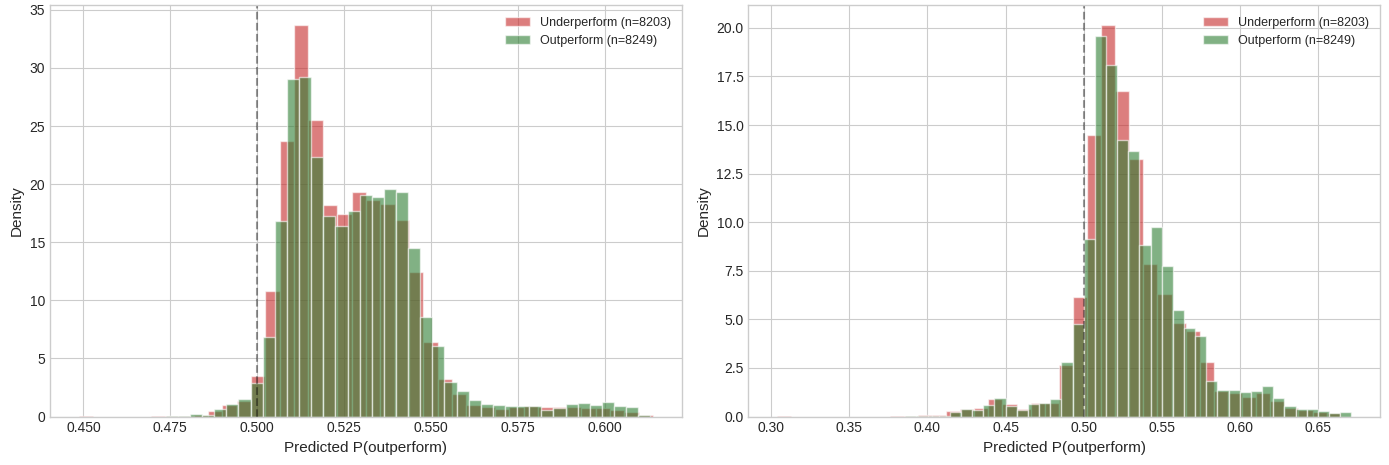
\includegraphics[width=\linewidth]{figs/prob_dist.png}
\caption{Distribution of validation-set predicted probabilities for the random forest (left) and XGBoost (right), split by realised outcome. The dashed line marks $p=0.5$, below which the half-Kelly rule assigns no weight.}
\label{fig:probs}
\end{figure}

\begin{figure}[t]
\centering
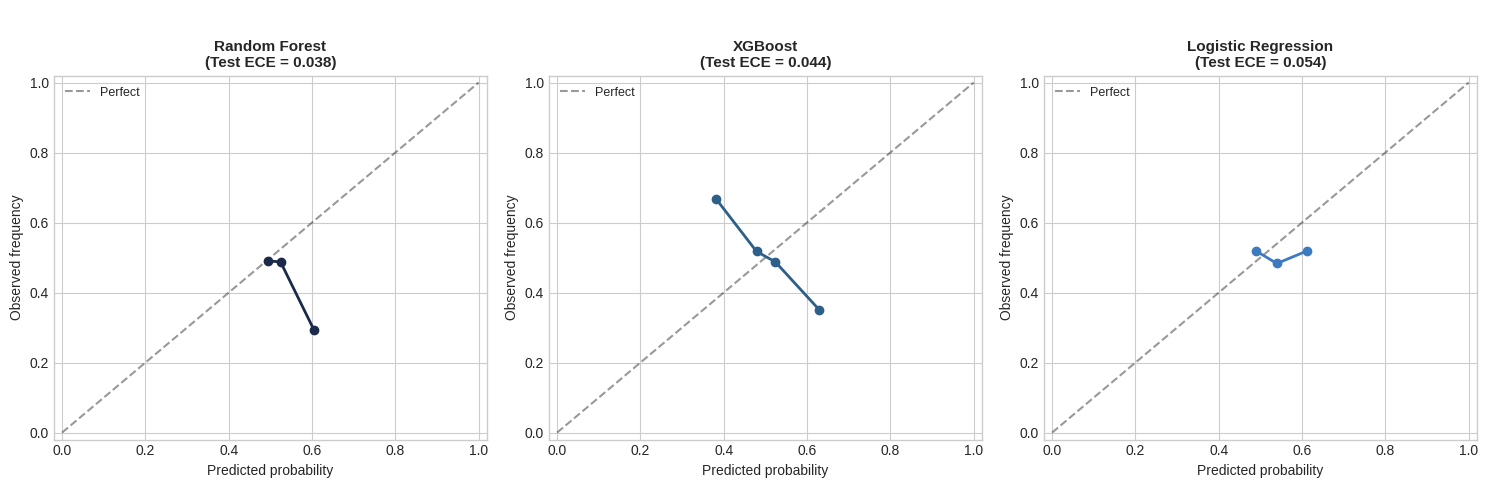
\includegraphics[width=\linewidth]{figs/test_reliability.png}
\caption{Test-set reliability diagrams for the three best-calibrated models. Points show the observed outperformance rate against the mean predicted probability in each occupied bin; the dashed line is perfect calibration.}
\label{fig:rel}
\end{figure}

\subsection{Portfolio performance}\label{sec:portfolio}

Table~\ref{tab:perf} reports the test-period performance. The calibration-selected portfolio returned 68.1\% over the four years, against 63.4\% for the accuracy-selected portfolio, with slightly lower volatility and a Sharpe ratio of 0.77 against 0.71. Under the arithmetic definition used for inference the corresponding figures are 0.81 and 0.76. The calibration-selected portfolio also had the deeper maximum drawdown, $-20.0\%$ against $-17.4\%$, so the higher return did not come with lower downside risk.

Neither model portfolio beat the simple benchmarks. The equal-weighted portfolio of the same 457 stocks returned 68.5\% with a Sharpe ratio of 0.82, and SPY returned 66.1\% with a Sharpe ratio of 0.83 and the lowest volatility of the four. The equity curves in Figure~\ref{fig:equity} track each other closely throughout the period, which is what one would expect from long-only portfolios drawn from the same universe with weights driven by a weak signal.

\begin{table}[t]
\centering\small
\caption{Test-period performance, January 2021 to December 2024 (48 months). Sharpe is compound annual return divided by annualised volatility, with a zero risk-free rate. Win rate is the share of months with a positive return.}
\label{tab:perf}
\begin{tabular}{@{}lcccccc@{}}
\toprule
Strategy & Total & Annual & Volatility & Sharpe & Max DD & Win rate \\
\midrule
Accuracy-selected (XGBoost) & 63.4\% & 13.1\% & 18.3\% & 0.71 & $-17.4\%$ & 60.4\% \\
Calibration-selected (random forest) & 68.1\% & 13.9\% & 18.1\% & 0.77 & $-20.0\%$ & 62.5\% \\
Equal weight (1/N) & 68.5\% & 13.9\% & 17.1\% & 0.82 & $-18.4\%$ & 58.3\% \\
SPY buy and hold & 66.1\% & 13.5\% & 16.3\% & 0.83 & $-24.0\%$ & 64.6\% \\
\bottomrule
\end{tabular}
\end{table}

\begin{figure}[t]
\centering
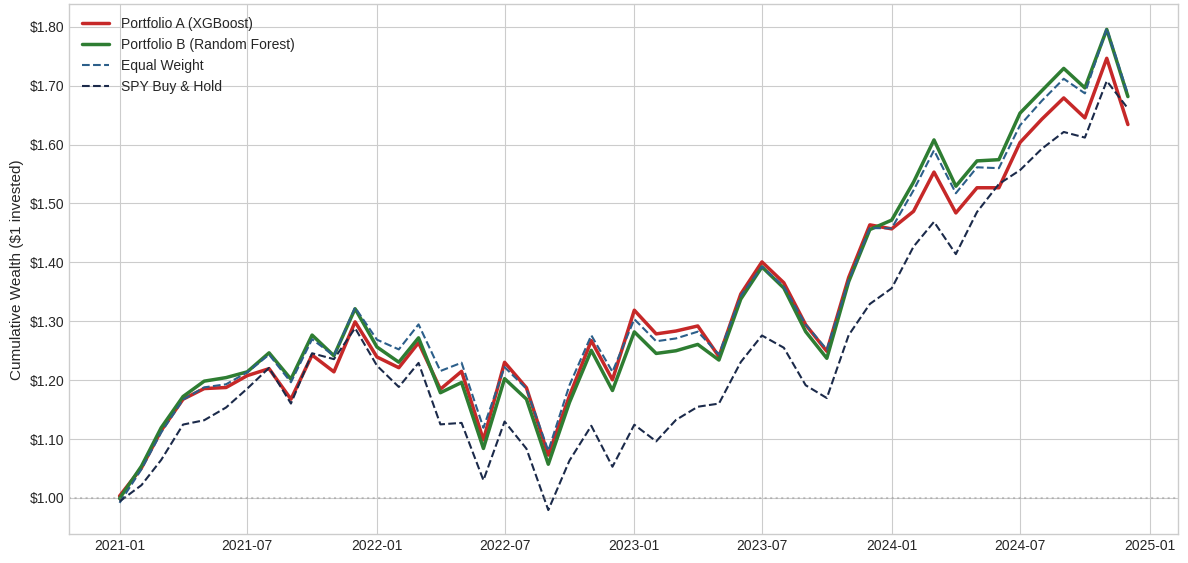
\includegraphics[width=0.85\linewidth]{figs/equity.png}
\caption{Cumulative value of one unit invested at the start of the test period.}
\label{fig:equity}
\end{figure}

\subsection{Inference}

Table~\ref{tab:stats} reports the tests of the primary hypothesis. The mean monthly return difference in favour of the calibration-selected portfolio is 0.057 percentage points. The paired $t$-statistic is 0.545 on 47 degrees of freedom, with a one-sided $p$-value of 0.294, and the standardised effect size is 0.080, well below the conventional threshold for a small effect. The differences are not normally distributed (Shapiro--Wilk $p=0.002$), so the $t$-test is approximate, but the bootstrap interval for the Sharpe difference, which does not rely on normality, also contains zero. The hypothesis is not supported at any conventional level, with or without the Bonferroni adjustment.

\begin{table}[t]
\centering\small
\caption{Tests of the primary hypothesis: calibration-selected minus accuracy-selected portfolio, 48 monthly returns.}
\label{tab:stats}
\begin{tabular}{@{}lll@{}}
\toprule
Test & Result & Reading \\
\midrule
Paired $t$-test (one-sided) & $t(47)=0.545$, $p=0.294$ & Not significant \\
Cohen's $d$ & 0.080 & Below a small effect (0.20) \\
Bootstrap 95\% interval, Sharpe difference & $[-0.080,\;0.204]$ & Contains zero \\
Bonferroni threshold & $\alpha=0.025$ & Not met \\
Shapiro--Wilk on differences & $W=0.911$, $p=0.002$ & Non-normal \\
\bottomrule
\end{tabular}
\end{table}

A sample of 48 months has little power for a test of this kind. Under the observed standard deviation of the monthly differences, an effect of the observed size would need several hundred months of data to reach conventional significance. The honest reading is that the experiment cannot rule out a small benefit from calibration, and that it gives no evidence of one.

\subsection{Feature ablation}

Removing the Elo pillar raises validation ECE from 0.0264 to 0.0291, and removing the Bayesian pillar raises it to 0.0275 (Table~\ref{tab:ablation}). Removing the technical pillar raises it to 0.0281, and removing the macroeconomic pillar lowers it slightly, to 0.0252. These changes are in the third decimal place, come from a single training run per configuration, and have no attached uncertainty. They suggest that the Elo and shrinkage features do not harm calibration, but they are not strong enough to claim that either pillar improves it.

\begin{table}[t]
\centering\small
\caption{Pillar ablation on the validation set, random forest.}
\label{tab:ablation}
\begin{tabular}{@{}lccc@{}}
\toprule
Configuration & Features & Validation ECE & Change \\
\midrule
Full model & 20 & 0.0264 & \\
Without technical & 12 & 0.0281 & $+0.0018$ \\
Without Elo & 16 & 0.0291 & $+0.0027$ \\
Without Bayesian & 17 & 0.0275 & $+0.0012$ \\
Without macroeconomic & 15 & 0.0252 & $-0.0012$ \\
\bottomrule
\end{tabular}
\end{table}

\subsection{Sensitivity to implementation choices}

To see how much the calibration-selected result depends on particular settings, the backtest was repeated 1{,}000 times with three perturbations drawn at random in each run: Gaussian noise with standard deviation 0.02 added to every predicted probability, a transaction cost drawn uniformly between 5 and 20 basis points, and a cap on the number of holdings drawn from 20, 50, 100 and 500. Across these runs the median total return was 63.5\%, the median maximum drawdown was $-21.1\%$ and the median arithmetic Sharpe ratio was 0.73; every run produced a positive total return. The point estimate in Table~\ref{tab:perf} is therefore somewhat favourable to the calibration-selected portfolio relative to nearby implementations. This exercise varies the implementation, not the market path, and should not be read as a forecast distribution.

\section{Discussion}

The hypothesis rests on a chain of reasoning: Kelly sizing turns probabilities into stakes, so better probabilities should give better stakes. The chain breaks at the first link when the model has almost no ability to separate winners from losers. In that regime a well-calibrated model is one that predicts close to the base rate for nearly every stock, and its ECE is low because it says little. The half-Kelly weights it produces are then driven by small differences in $\hat{p}$ around 0.5, which carry little information about returns. A calibration-selected model is still preferable to a badly calibrated one, as the multilayer perceptron shows, but among reasonable models the selection criterion makes little economic difference.

Two implications follow for practice. First, calibration should be evaluated jointly with resolution. The Brier decomposition \citep{murphy1973} separates the two, and a model with near-zero resolution should not be preferred for its reliability alone. Second, the benchmark matters. Against a zero return or a market index with a deep drawdown, both model portfolios would have looked successful. Against equal weighting of the same universe, neither added value, which is consistent with \citet{demiguel2009}.

\section{Limitations}

\begin{itemize}
  \item \textbf{Survivorship bias.} The universe is a single recent snapshot of index membership, so it excludes firms that left the index before the snapshot date. This typically flatters returns by an amount on the order of 50 to 100 basis points a year. It affects all four strategies, but not necessarily equally.
  \item \textbf{Macroeconomic revisions.} FRED series are used in their current revised form rather than as real-time vintages. The one-month lag removes the most obvious look-ahead but not the effect of later revisions.
  \item \textbf{Single path, short test period.} The test covers 48 months of one market regime, and the models are trained once with one random seed. The statistical power to detect a modest difference is low.
  \item \textbf{Limited tuning.} Ten Optuna trials per model is a small budget. A larger search could change which model is calibration-best or accuracy-best.
  \item \textbf{Collinearity.} Variance inflation factors are very high within the Elo pillar (maximum about 2{,}800), because its four features share one update rule. This does not bias tree-based predictions but limits any interpretation of individual features.
  \item \textbf{Benchmark costs.} The equal-weight and SPY benchmarks are not charged transaction costs. Charging them would narrow, but on these figures not reverse, the benchmarks' advantage.
  \item \textbf{Data access.} The price data were obtained from a free public source. I was not able to rerun the download for this version of the paper, so the results reported here are those of the archived run in the replication repository.
\end{itemize}

Several extensions would strengthen the analysis: rerunning across multiple random seeds and tuning budgets; a Wilcoxon signed-rank test alongside the $t$-test; the \citet{ledoit2008} test for the difference of two Sharpe ratios; a deflated Sharpe ratio \citep{bailey2014}; a point-in-time constituent list; and post-hoc recalibration of the accuracy-selected model, which would test whether a recalibrated accurate model can match a model selected for calibration.

\section{Conclusion}

Selecting a return classifier for calibration rather than accuracy produced a portfolio that earned more over 2021 to 2024, but the difference was small, not statistically significant, and neither portfolio beat an equal-weighted portfolio of the same stocks. The reason is that both models had almost no discriminating power, so calibration error measured caution more than insight. Calibration remains a necessary property when probabilities size positions, but on this evidence it is not a source of return in its own right. It becomes valuable only once the model has something to say.

\section*{Reproducibility and disclosure}

All code, executed notebooks, figures and tables are available at \url{https://github.com/pablowilliams/calibration-portfolio}. Figures in this paper are taken from that run. An earlier written description of the portfolio rule referred to an equal-weighted top-quintile selection with 5 basis points per leg; the code that produced every reported result uses the half-Kelly rule and 10 basis points on turnover described in Section~\ref{sec:construction}, and this paper describes the code as executed. The author used an AI coding assistant (Claude, Anthropic) during software development. All modelling decisions, temporal-leakage checks and interpretation of results are the author's, and the collaboration log is included in the repository. The author received no funding for this work and declares no conflicts of interest.

\begin{thebibliography}{99}
\bibitem[Akiba et~al.(2019)]{akiba2019} Akiba, T., Sano, S., Yanase, T., Ohta, T. and Koyama, M. (2019). Optuna: A next-generation hyperparameter optimization framework. \emph{Proceedings of the 25th ACM SIGKDD International Conference on Knowledge Discovery and Data Mining}, 2623--2631.
\bibitem[Bailey and L\'opez de Prado(2014)]{bailey2014} Bailey, D.~H. and L\'opez de Prado, M. (2014). The deflated Sharpe ratio: Correcting for selection bias, backtest overfitting, and non-normality. \emph{Journal of Portfolio Management}, 40(5), 94--107.
\bibitem[Breiman(2001)]{breiman2001} Breiman, L. (2001). Random forests. \emph{Machine Learning}, 45(1), 5--32.
\bibitem[Brier(1950)]{brier1950} Brier, G.~W. (1950). Verification of forecasts expressed in terms of probability. \emph{Monthly Weather Review}, 78(1), 1--3.
\bibitem[Chen and Guestrin(2016)]{chen2016} Chen, T. and Guestrin, C. (2016). XGBoost: A scalable tree boosting system. \emph{Proceedings of the 22nd ACM SIGKDD International Conference on Knowledge Discovery and Data Mining}, 785--794.
\bibitem[DeMiguel et~al.(2009)]{demiguel2009} DeMiguel, V., Garlappi, L. and Uppal, R. (2009). Optimal versus naive diversification: How inefficient is the 1/N portfolio strategy? \emph{Review of Financial Studies}, 22(5), 1915--1953.
\bibitem[Efron and Morris(1977)]{efron1977} Efron, B. and Morris, C. (1977). Stein's paradox in statistics. \emph{Scientific American}, 236(5), 119--127.
\bibitem[Elo(1978)]{elo1978} Elo, A.~E. (1978). \emph{The Rating of Chessplayers, Past and Present}. New York: Arco.
\bibitem[Gu et~al.(2020)]{gu2020} Gu, S., Kelly, B. and Xiu, D. (2020). Empirical asset pricing via machine learning. \emph{Review of Financial Studies}, 33(5), 2223--2273.
\bibitem[Guo et~al.(2017)]{guo2017} Guo, C., Pleiss, G., Sun, Y. and Weinberger, K.~Q. (2017). On calibration of modern neural networks. \emph{Proceedings of the 34th International Conference on Machine Learning}, 1321--1330.
\bibitem[Harvey et~al.(2016)]{harvey2016} Harvey, C.~R., Liu, Y. and Zhu, H. (2016). \ldots and the cross-section of expected returns. \emph{Review of Financial Studies}, 29(1), 5--68.
\bibitem[Kelly(1956)]{kelly1956} Kelly, J.~L. (1956). A new interpretation of information rate. \emph{Bell System Technical Journal}, 35(4), 917--926.
\bibitem[Ledoit and Wolf(2008)]{ledoit2008} Ledoit, O. and Wolf, M. (2008). Robust performance hypothesis testing with the Sharpe ratio. \emph{Journal of Empirical Finance}, 15(5), 850--859.
\bibitem[L\'opez de Prado(2018)]{lopezdeprado2018} L\'opez de Prado, M. (2018). \emph{Advances in Financial Machine Learning}. Hoboken, NJ: Wiley.
\bibitem[MacLean et~al.(2011)]{maclean2011} MacLean, L.~C., Thorp, E.~O. and Ziemba, W.~T. (eds.) (2011). \emph{The Kelly Capital Growth Investment Criterion: Theory and Practice}. Singapore: World Scientific.
\bibitem[Murphy(1973)]{murphy1973} Murphy, A.~H. (1973). A new vector partition of the probability score. \emph{Journal of Applied Meteorology}, 12(4), 595--600.
\bibitem[Naeini et~al.(2015)]{naeini2015} Naeini, M.~P., Cooper, G.~F. and Hauskrecht, M. (2015). Obtaining well calibrated probabilities using Bayesian binning. \emph{Proceedings of the 29th AAAI Conference on Artificial Intelligence}, 2901--2907.
\bibitem[Niculescu-Mizil and Caruana(2005)]{niculescu2005} Niculescu-Mizil, A. and Caruana, R. (2005). Predicting good probabilities with supervised learning. \emph{Proceedings of the 22nd International Conference on Machine Learning}, 625--632.
\bibitem[Platt(1999)]{platt1999} Platt, J. (1999). Probabilistic outputs for support vector machines and comparisons to regularized likelihood methods. In \emph{Advances in Large Margin Classifiers}, 61--74. Cambridge, MA: MIT Press.
\bibitem[Thorp(2006)]{thorp2006} Thorp, E.~O. (2006). The Kelly criterion in blackjack, sports betting, and the stock market. In \emph{Handbook of Asset and Liability Management}, Vol.~1, 385--428. Amsterdam: Elsevier.
\bibitem[Zadrozny and Elkan(2002)]{zadrozny2002} Zadrozny, B. and Elkan, C. (2002). Transforming classifier scores into accurate multiclass probability estimates. \emph{Proceedings of the 8th ACM SIGKDD International Conference on Knowledge Discovery and Data Mining}, 694--699.
\end{thebibliography}

\end{document}
